% !TEX root = presentation.tex
	\begin{frame}
		\frametitle{Geometry}
		\todo[inline]{Bezier and Bernstein recap/why cubic?}
	\end{frame}

	% Geometry process
	\begin{frame}\frametitle{Geometry - step 1}
		\missingfigure{Flat triangle picture, with uniform distributed control points}
		\begin{equation*}
			b_{ijk} = (iP_1 + jP_2 + kP_3)/3
		\end{equation*}
	\end{frame}

	\begin{frame}\frametitle{Geometry - step 2}
		\missingfigure{Figure 6 of the paper}
	\end{frame}

	\begin{frame}\frametitle{Geometry - step 3}
		\missingfigure{Figure 3 with center down.}
	\end{frame}	

	\begin{frame}\frametitle{Geometry - result}
		% \todo[inline]{How do you create the PN triangle geometrically}
		\begin{columns}
			\begin{column}{0.6\textwidth}
				\begin{center}
				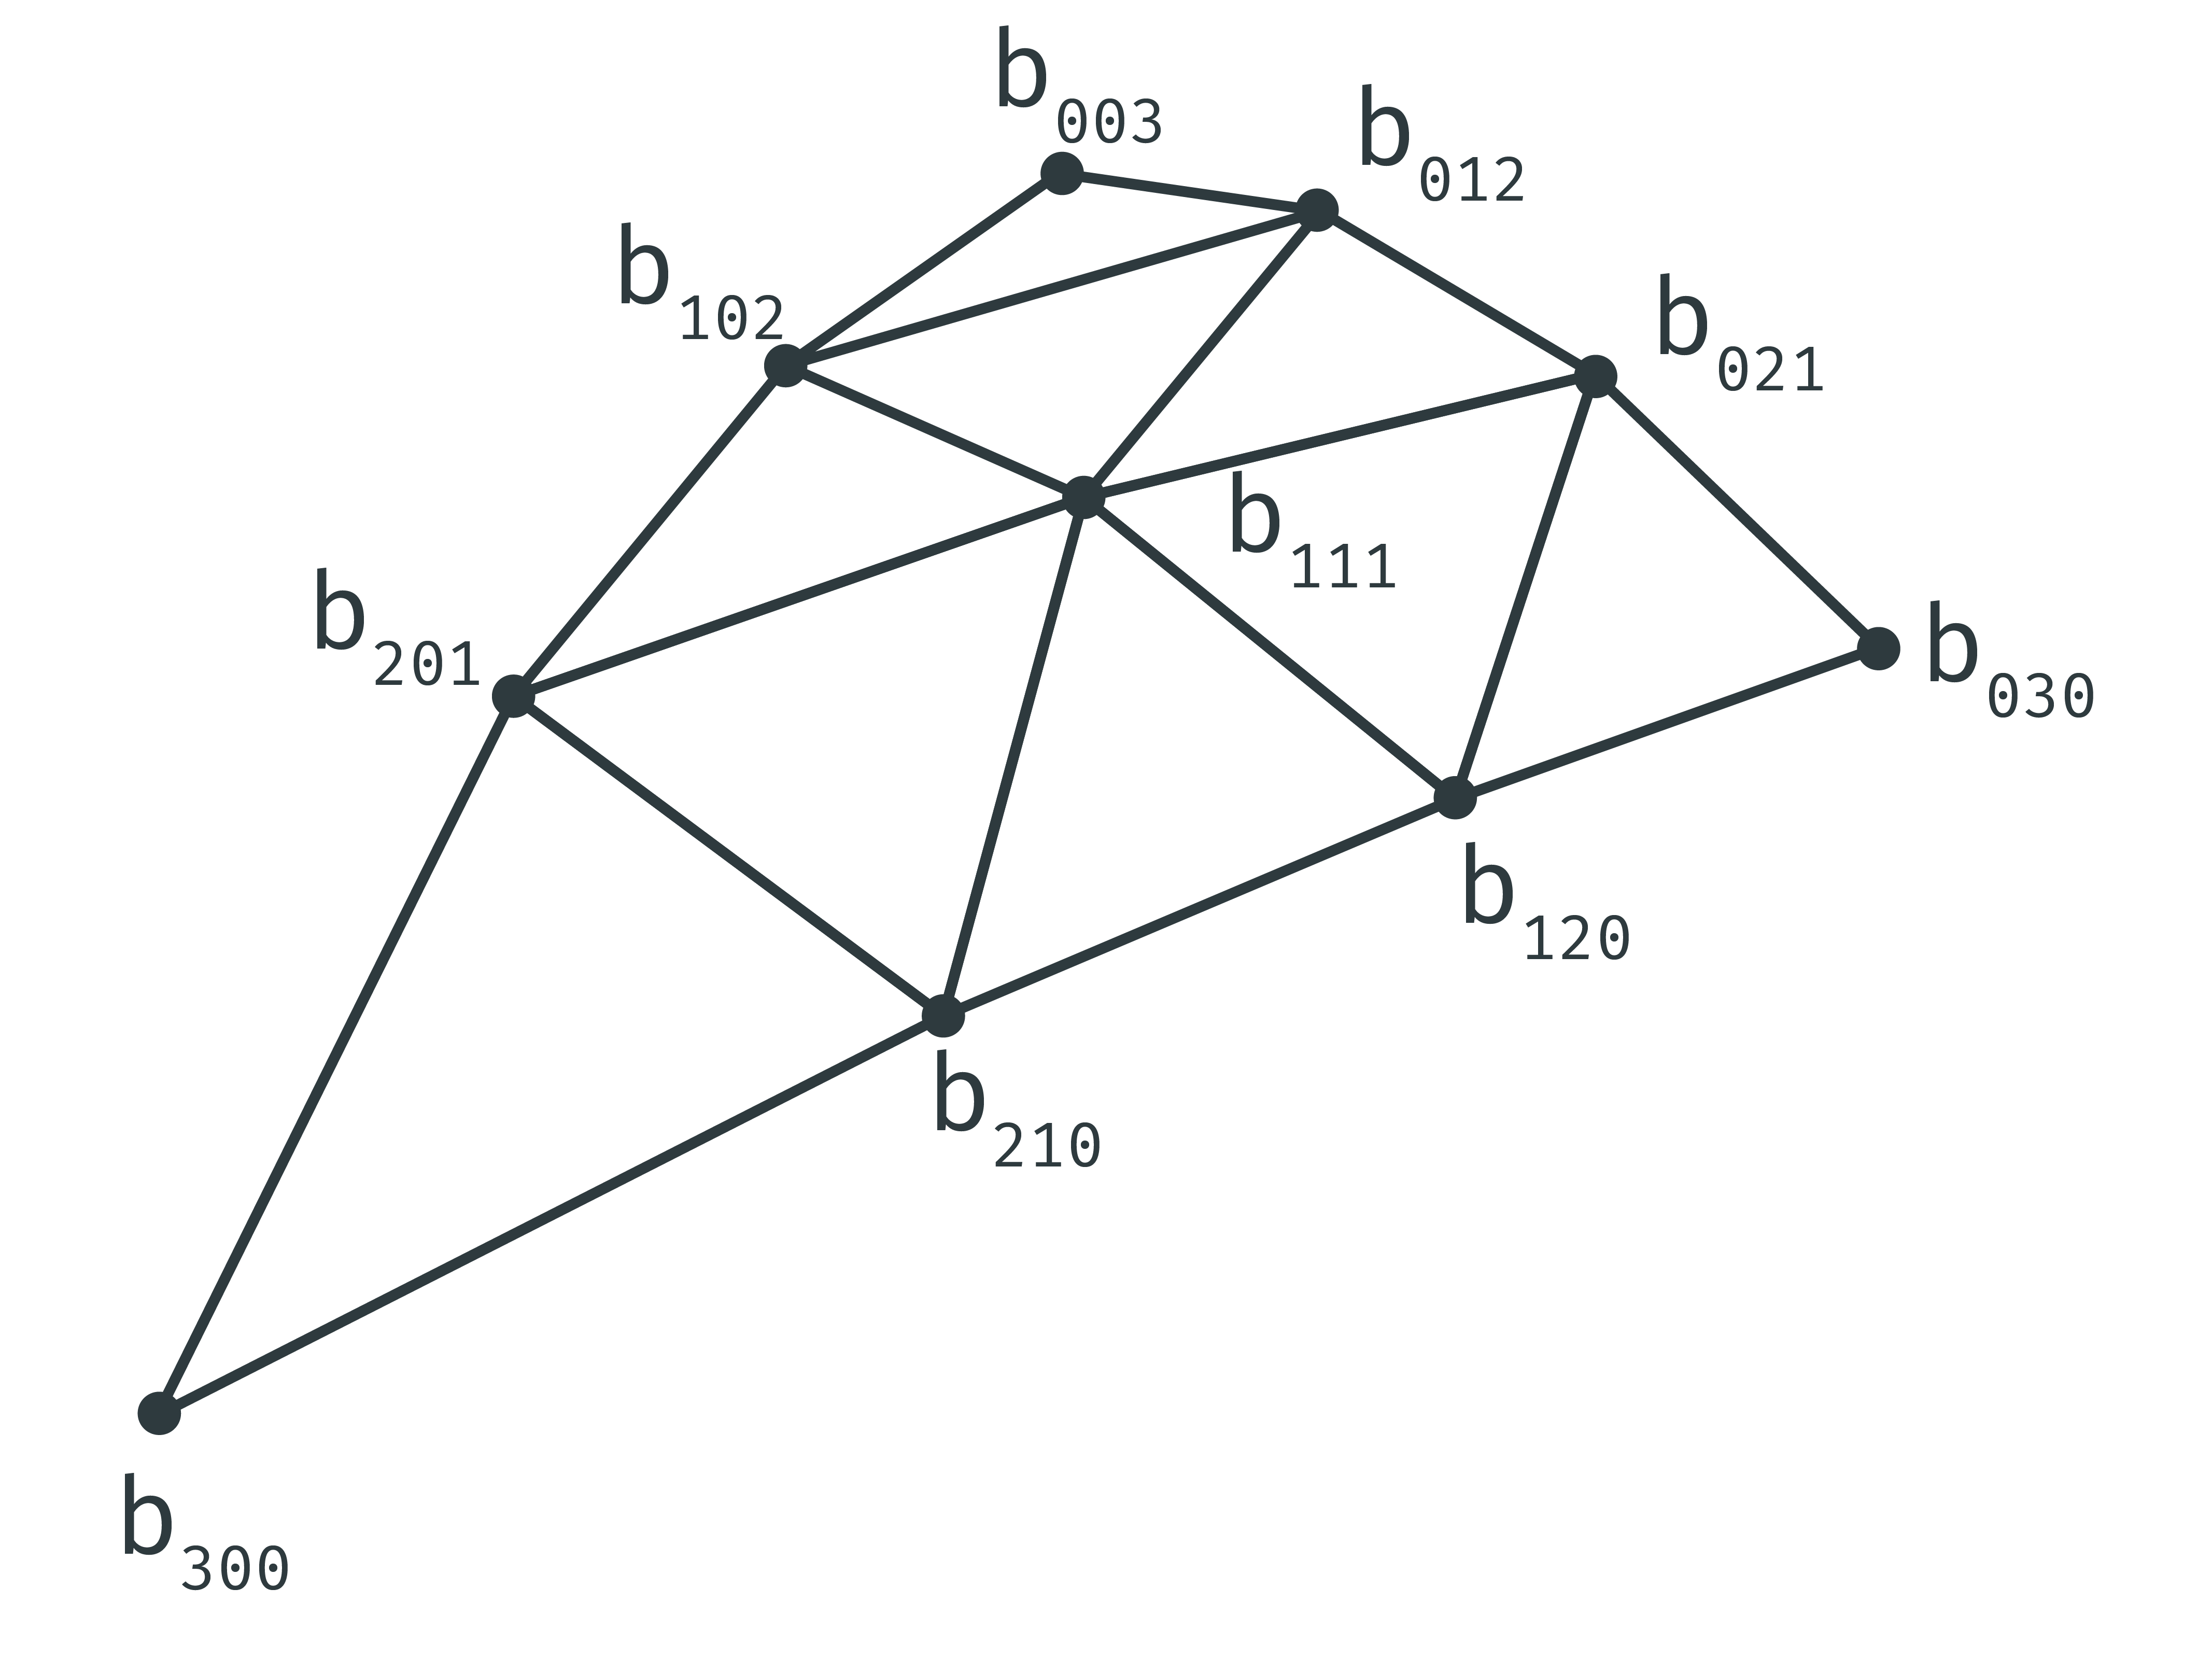
\includegraphics[width=\textwidth]{img/1_single/geometry_4.png}
				\end{center}	
			\end{column}
			\begin{column}{0.4\textwidth}
				\begin{equation*}
					A^2 + B^2 = C^2
				\end{equation*}
			\end{column}
		\end{columns}
	\end{frame}

	\begin{frame}
		\frametitle{Normals}
		\todo[inline]{How do you create the PN triangle normals}
	\end{frame}

	\begin{frame}
		\frametitle{Normals}
		\todo[inline]{Quadratic why no linear / cubic}
	\end{frame}

	\begin{frame}
		\frametitle{Level Of Detail}
		\todo[inline]{Barycentric coordinates recap}
	\end{frame}	

	\begin{frame}
		\frametitle{Level Of Detail}
		\todo[inline]{LOD verhaal}
		\begin{columns}
			\begin{column}[b]{0.22\textwidth}
				\begin{center}
					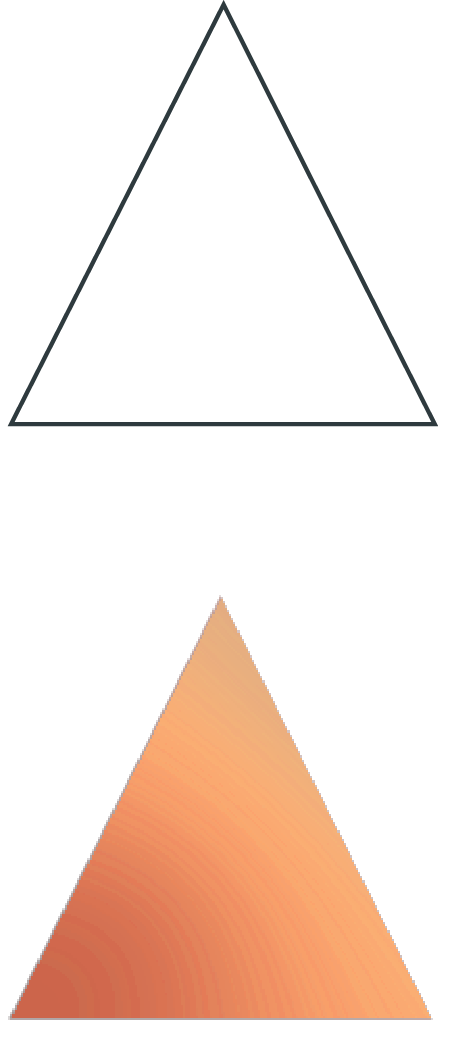
\includegraphics[width=\textwidth]{./img/1_single/lod_lod0.png}
					\small{0}
				\end{center}	
			\end{column}
			\begin{column}[b]{0.22\textwidth}
				\begin{center}
					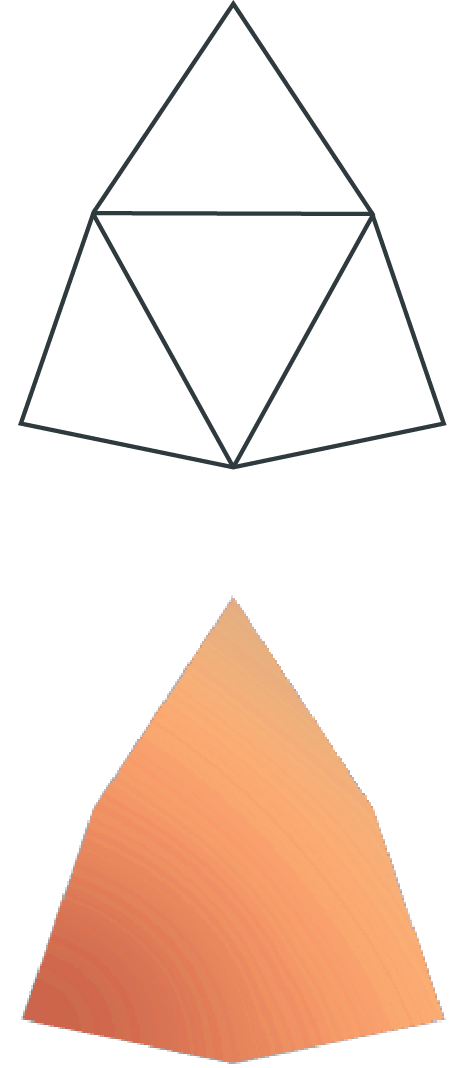
\includegraphics[width=\textwidth]{./img/1_single/lod_lod1.png}	
					\small{1}
				\end{center}	
			\end{column}
			\begin{column}[b]{0.22\textwidth}
				\begin{center}
					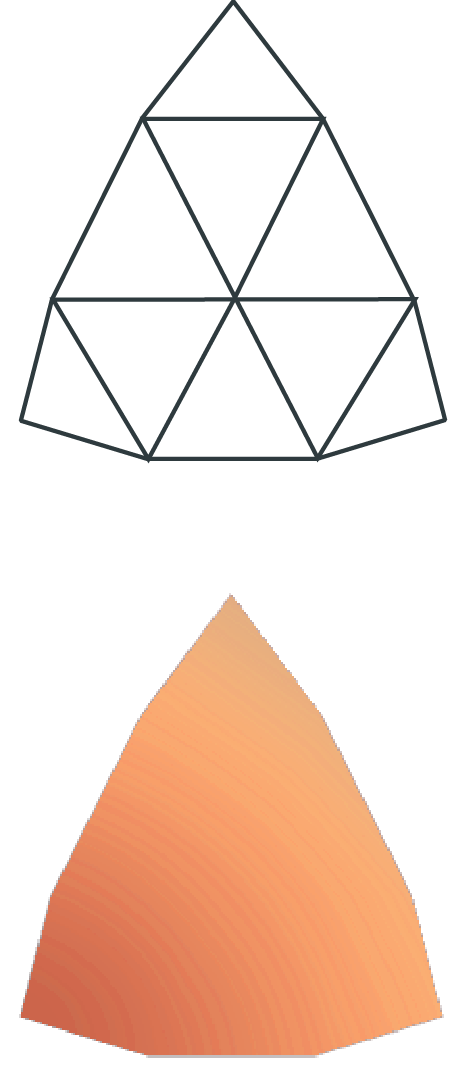
\includegraphics[width=\textwidth]{./img/1_single/lod_lod2.png}	
					\small{2}
				\end{center}	
			\end{column}
			\begin{column}[b]{0.22\textwidth}
				\begin{center}
					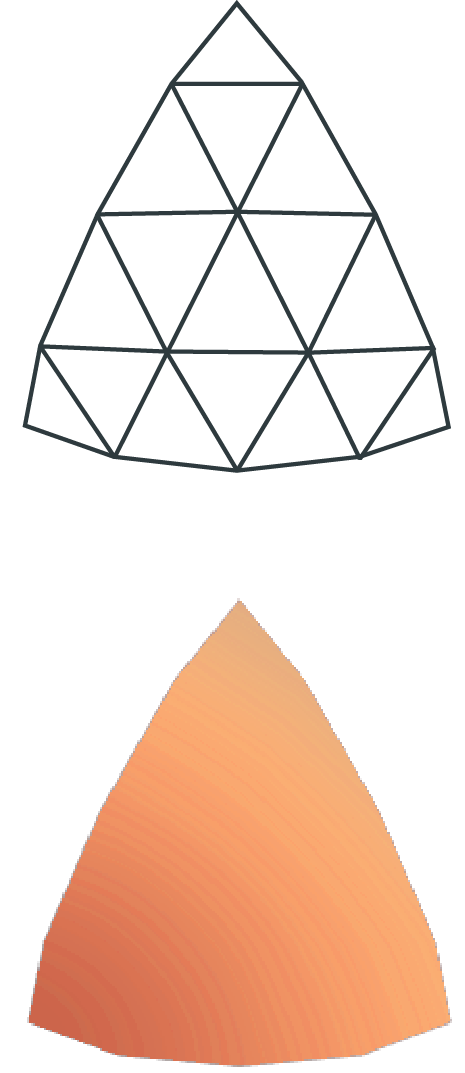
\includegraphics[width=\textwidth]{./img/1_single/lod_lod3.png}	
					\small{3}
				\end{center}	
			\end{column}
		\end{columns}
	\end{frame}	

	\begin{frame}
		\frametitle{Construction}
		\todo[inline]{The steps. Recap of everything construct geometry and normals and evaluate less (low lod) or more points (high lod)}
	\end{frame}	